\documentclass[main.tex]{subfiles}
\begin{document}

\section{Topologie in metrische ruimten}
\label{sec:topol-metr-ruimt}

\subsection{Open en gesloten verzamelingen}
\label{sec:open-en-gesloten}
hello it is i leclerc
\begin{de}
  Zij $V,d$ een metrische ruimte, dan noemen we een deelverzameling $W$ van $V$ \term{open} als het volgende geldt:
  \[ \forall v\in W, \exists \delta \in \mathbb{R}_{0}^{+}, \forall w\in W:\ d(v,w) < \delta \Rightarrow w \in W \]
\end{de}

\begin{de}
  Zij $V,d$ een metrische ruimte, dan noemen we een deelverzameling $W$ van $V$ \term{gesloten} als het complement $V\setminus W$ van $W$ in $V$ open is.
\end{de}

\begin{de}
  Zij $V,d$ een metrische ruimte, $x\in V$ en $\delta \in \mathbb{R}_{0}^{+}$, dan noemen we de verzameling $B(x,\delta)$ als volgt, de \term{open bol} met middelpunt $x$ en straal $\delta$.
  \[ B(x,\delta) = \{ y\in V \mid d(x,y) < \delta \} \]
\end{de}

\begin{de}
  Zij $V,d$ een metrische ruimte, $x\in V$ en $\delta \in \mathbb{R}_{0}^{+}$, dan noemen we de verzameling $B\interval{x}{\delta}$ als volgt, de \term{gesloten bol} met middelpunt $x$ en straal $\delta$.
  \[ B(x,\delta) = \{ y\in V \mid d(x,y) \le \delta \} \]
\end{de}

\begin{st}
  Een open bol $B(x,\delta)$ in een metrische ruimte $V,d$ is een open deelverzameling van $V$.

  \begin{proof}
    Kies een willekeurig punt $y\in V$ met $d(x,y) < \delta$ en kies $\epsilon = \delta - d(x,y)$.
    Kies een willekeurig punt $z\in B(y,\epsilon)$, dan geldt het volgende:
    \[ d(x,z) \le d(x,y) + d(y,z) < d(x,y) + \epsilon = d(x,y) + \delta - d(x,y) = \delta \]
    Er bestaat dus steeds een open bol binnen $B(x,\delta)$ die er deel van uitmaakt.
  \end{proof}
\end{st}

\begin{st}
  Een gesloten bol $B\interval{x}{\delta}$ in een metrische ruimte $V,d$ is een gesloten deelverzameling van $V$.

  \begin{proof}
    We bewijzen dat $X = V \setminus B\interval{x}{\delta}$ open is.
    Kies willekeurig een $z\in X$ en noem $\epsilon = d(x,z) - \delta$.
    Kies een willekeurig punt $y\in B(z,\epsilon)$, dan geldt het volgende:
    \[ d(x,y) \ge d(x,z) - d(y,z) > d(x,z) - \epsilon = d(x,z) -d(x,z) + \delta = \delta \]
    Er bestaat dus een open bol rond elk punt $x$ buiten $B\interval{x}{\delta}$ die volledig buiten $B\interval{x}{\delta}$ ligt.
  \end{proof}
\end{st}



\begin{pr}
  Zij $V,d$ een metrische ruimte, dan is de unie van open verzamelingen in $V$ ook open in $V$.

  \begin{proof}
    Zij $\mathcal{O}$ een niet-lege verzameling van open deelverzamelingen van $V$.
    Noem $U = \bigcup_{A\in \mathcal{O}}A$.
    \begin{itemize}
    \item Als $U$ leeg is, is $U$ trivialerwijs open.
    \item Als $U$ niet leeg is, dan bestaat er een $a$ in een $A \subseteq \mathcal{O}$ als volgt:
      \[ \forall v\in A, \exists \delta \in \mathbb{R}_{0}^{+}, \forall w\in V:\ d(v,w) < \delta \Rightarrow w \in A \]
      Omdat $A$ een deel is van $U$, zal hetzelfde gelden voor $U$.
    \end{itemize}
  \end{proof}
\end{pr}

\begin{pr}
  Zij $V,d$ een metrische ruimte, dan is een \textbf{eindige} doorsnede van open verzamelingen in $V$ ook open in $V$.
  
  \begin{proof}
    Beschouw een eindig aantal ($n$) open deelverzamelingen $A_{i}$ van $V$.
    Noem $D = \bigcap_{i}A_{x}$.
    \begin{itemize}
    \item Als $D$ leeg is, is $D$ trivialerwijs open.
    \item Als $D$ niet leeg is, dan bestaat er een $a\in D$ als volgt:
      \[ \forall i, \exists \delta_{i} \in \mathbb{R}_{0}^{+}, \forall w\in V:\ d(a,w) < \delta \Rightarrow w \in A_{i} \]
      Kies nu $\delta = \min_{i}\delta_{i}$, dan geldt het volgende:
      \[ \forall w\in V:\ d(a,w) < \delta \Rightarrow w\in D \]
    \end{itemize}
  \end{proof}
\end{pr}

\begin{opm}
  Deze stelling geldt niet voor een oneindige doorsnede van verzamelingen omdat $\min_{i}\delta_{i}$ dan niet noodzakelijk bestaat.
\end{opm}
\extra{tegenvoorbeeld}

\begin{pr}
  Een doorsnede van gesloten verzamelingen is gesloten.
\extra{bewijs}
\end{pr}

\begin{pr}
  Een \textbf{eindige} unie van gesloten verzamelingen is gesloten
\extra{bewijs}
\end{pr}

\begin{pr}
  \label{pr:metrische-ruimte-gesloten-itv-rijen}
  Zij $V,d$ een metrische ruimte en $A$ een niet-leeg deel van $V$, dan is $A$ gesloten als en slechts als de limiet van elke convergente rij in $A$ ook tot $A$ behoort.

  \begin{proof}
    Bewijs van een equivalentie.
    \begin{itemize}
    \item $\Rightarrow$\\
      Kies een willekeurige convergente rij $(x_{n})_{n}$ in $A$ en noem de limiet $x$.
      Veronderstel dat $x$ niet tot $A$ zou behoren, dan behoort $x$ tot het open deel $V \setminus A$ van $V$.
      We kunnen dus een $\delta \in \mathbb{R}_{0}^{+}$ vinden als volgt:
      \[ \forall w \in A:\ d(x,w) < \delta \Rightarrow w \in V \setminus A \]
      Omdat $x$ de limiet is van $(x_{n})_{n}$, kunnne we eveneens een $n_{0}\in \mathbb{N}$ vinden als volgt:
      \[ \forall n\in \mathbb{N}:\ n \ge n_{0} \Rightarrow d(x_{n},x) < \delta \]
      Nemen we deze beweringen samen, dan bestaat er minstens \'e\'en $x_{n}$ met $n\ge n_{0}$ in $V \setminus A$.
      Contridictie.
    \item $\Leftarrow$\\
      Bewijs uit het ongerijmde: Stel dat $A$ niet gesloten is.
      $A^{c}$ is dan niet open en er bestaat dus een $a\in V \setminus A$ als volgt:
      \[ \forall \delta \in \mathbb{R}_{0}^{+}, \exists b\in V:\ d(a,b) < \delta \wedge b \in A \]
      We kunnen een rij construeren door voor $\delta_{n}$ telkens $\frac{1}{n}$ te kiezen en zo een $x_{n}$ te bekomen.
      Per constructie geldt voor elke $n\in \mathbb{N}$ dan $d(x_{n},a) < \frac{1}{n}$ en zal de rij dus naar $a$ convergeren.
      We hebben nu een convergente rij $(x_{n})_{n}$ in $A$ geconstrueerd waarvoor de limiet niet tot $A$ behoort.
      Contradictie.
    \end{itemize}
  \end{proof}
\end{pr}

\subsection{Topologie\"en}
\label{sec:topologieen}

\begin{de}
  Zij $X$ verzameling en $d$ een metriek op $X$, dan noemen we de verzameling $\mathcal{T}_{d}$ van $d$-open delen van $X$ de (metrische) \term{topologie} ge\"induceerd door $d$ op $X$.
\end{de}

\begin{de}
  Zij $d_{1}$ en $d_{2}$ twee metrieken op een verzameling $X$.
  We noemen $d_{1}$ \term{topologisch fijner} dan $d_{2}$ als $\mathcal{T}_{d_{1}}$ een deel is van $\mathcal{T}_{d_{2}}$:
  T.t.z als elk $d_{2}$-open deel van $X$ ook $d_{1}$-open is.
\end{de}

\question{is 'topologisch fijner' een totale ordeverzameling?}

\begin{de}
  We noemen twee metrieken $d_{1}$ en $d_{2}$ \term{topologisch equivalent} als $\mathcal{T}_{d_{1}}$ en $\mathcal{T}_{d_{2}}$ gelijk zijn.
\end{de}

\begin{st}
  Zij $X$ een niet-lege verzameling en $d_{1}$ en $d_{2}$ metrieken op $X$, dan zijn volgende uitspraken equivalent.
  \begin{enumerate}
  \item $d_{1}$ is topologisch fijner dan $d_{2}$.
  \item Binnen elke $d_{2}$-open bol ligt er een $d_{1}$-open bol met hetzelfde middelpunt:
    \[ \forall x\in X, \forall r \in \mathbb{R}_{0}^{+}, \exists r' \in \mathbb{R}_{0}^{+}:\ B_{1}(x,r') \subseteq B_{2}(x,r) \]
  \item De identieke afbeelding $\mathfrak{i}:\ X,d_{1} \rightarrow X,d_{2}:\ x \mapsto x$ is continu.
  \item Voor elke rij $(x_{n})_{n}$ in $X$ en elke $a\in X$: geldt de volgende implicatie:
    \[ x_{n} \overset{d_{1}}{\rightarrow} a \Rightarrow x_{n} \overset{d_{2}}{\rightarrow} a \]
  \end{enumerate}

  \begin{proof}
    Bewijs van equivalentie met circulaire implicaties.
    \begin{itemize}
    \item $(1) \Rightarrow (2)$\\
      Kies willekeurig een $x \in X$ en een $r\in \mathbb{R}_{0}^{+}$.
      $B_{d_{2}}(x,r)$ is dan een open bol voor $d_{2}$, maar ook $d_{1}$ open (,hoewel dan niet noodzakelijk een bol,) omdat $d_{1}$ topologisch fijner is dan $d_{2}$.
      Nu is $x$ ook een element van $B_{d_{2}}(x,r)$ en dus bestaat er een $r'\in \mathbb{R}_{0}^{+}$ zodat $B_{d_{1}}(x,r')$ een deel is van $B_{d_{2}}(x,r)$.
    \item $(2) \Rightarrow (3)$\\
      Kies een willekeurige $x\in X$ en een $\epsilon \in \mathbb{R}_{0}^{+}$.
      We kunnen dan een $\delta \in \mathbb{R}_{0}^{+}$ vinden zodat $B_{d_{1}}(x,\delta)$ een deel is van $B_{d_{2}}(x,\epsilon)$.
      Nu volgt de implicatie direct:
      \[ \forall x,y\in X:\ d_{1}(x,y) < \delta \Rightarrow d_{2}(\mathfrak{i}(x),\mathfrak{i}(y)) = d(x,y) < \epsilon \]
    \item $(3) \Rightarrow (4)$\\
      Kies willekeurig een rij $(x_{n})_{n}$ in $X$ met een $a\in X$ als limiet voor $d_{1}$.
      We tonen aan dat $(x_{n})_{n}$ ook voor $d_{2}$ naar $a$ convergeert.
      Kies daartoe een $\epsilon \in \mathbb{R}_{0}^{+}$.
      Omdat $\mathfrak{i}$ continu is in $a$, kunnen we een $\delta \in \mathbb{R}_{0}^{+}$ vinden als volgt:
      \[ \forall x\in X:\ d_{1}(x,a) < \delta \Rightarrow d_{2}(x,a) < \epsilon \]
      Omdat $(x_{n})_{n}$ naar $a$ convergeert, kunnen we dus een $n_{0}\in \mathbb{N}$ vinden zodat het volgende geldt:
      \[ \forall n\in \mathbb{N}:\ n \ge n_{0} \Rightarrow d_{1}(x_{n},a) < \delta \]
      Vanaf die $n$ zal dus ook $d_{2}(x_{n},a)$ kleiner zijn dan $\epsilon$.
      Hierin was $\epsilon$ willekeurig en dus convergeert $(x_{n})_{n}$ naar $a$.
    \item $(4) \Rightarrow (1)$\\
      We tonen aan dat elk $d_{2}$-open deel van $X$ ook $d_{1}$-open is.
      Dit is equivalent met aantonen dat elk $d_{2}$-gesloten deel van $X$ ook $d_{1}$ gesloten is.
      Kies dus een $d_{2}$ gesloten deel $A \subseteq X$.
      Als $A$ leeg is, is $A$ zeker $d_{1}$-gesloten.
      Veronderstel daarom dat $A$ niet leeg is en kies een willekeurige rij $(x_{n})_{n}$ in $X$ die convergeert naar $a$ voor $d_{1}$.
      $(x_{n})_{n}$ zal dan ook voor $d_{2}$ naar $a$ convergeren en omdat $A$ $d_{2}$-gesloten is moet $a$ daarom tot $A$ behoren.\prref{pr:metrische-ruimte-gesloten-itv-rijen}
    \end{itemize}
  \end{proof}
\end{st}

\begin{opm}
  Topologisch equivalente metrieken hebben dus dezelfde open bollen en dezelfde convergente rijen.
\end{opm}

\begin{opm}
  Ookal hebben topologisch equivalente metrieken dezelfde convergente rijen, ze kunnen nog steeds verschillende Cauchyrijen hebben.
  Voor twee topologisch equivalente metrieken kan $X,d_{1}$ dus volledig zijn zonder dat $X,d_{2}$ volledig is.\deref{de:metrische-ruimte-volledig}
\TODO{voorbeeld van zo'n situatie}
\end{opm}

\subsection{Sluiting en inwendige}
\label{sec:sluit-en-inwend}

\begin{de}
  Zij $X,d$ een metrische ruimte, dan noemen we de unie $\mathring{X}$ van alle open deelverzamelingen van een deelverzameling $W$ van $X$ het \term{inwendige} van $W$.
\end{de}

\begin{de}
  Zij $X,d$ een metrische ruimte, dan noemen we de doorsnede $\overline{X}$ van alle gesloten oververzamelingen van een deelverzameling $W$ van $X$ de \term{sluiting} van $W$.
\end{de}

\begin{pr}
  Zij $X,d$ een metrische ruimte en zij $A$ een deelverzameling van $X$, dan kunnen we $\mathring{W}$ als volgt beschrijven:
  \[ \mathring{A} = \{ x \in A \mid \exists \delta \in \mathbb{R}_{0}^{+}:\ B(x,\delta) \subseteq A \} \]
\TODO{bewijs}
\end{pr}

\begin{pr}
  Zij $X,d$ een metrische ruimte en zij $A$ een deelverzameling van $X$, dan kunnen we $\overline{A}$ als volgt beschrijven:
  \[ \overline{A} = \{ x\in A \mid \forall \delta \in \mathbb{R}_{0}^{+}:\ B(x,\delta) \cap A \neq \emptyset \} \]
\TODO{bewijs}
\end{pr}

\begin{de}
  We noemen een punt $x\in \mathring{A}$ in een deelverzameling $A$ van $X$ in een metrische ruimte $X,d$ \term{inwendig}.
  \[ \exists \delta \in \mathbb{R}_{0}^{+}:\ B(x,\delta) \subseteq A \]
\end{de}

\begin{de}
  We noemen een punt $x\in \overline{A}$ in een deelverzameling $A$ van $X$ in een metrische ruimte $X,d$ \term{adherent}.
  \[ \forall \delta \in \mathbb{R}_{0}^{+}:\ B(x,\delta) \cap A \neq \emptyset \]
\end{de}

\begin{pr}
  \label{pr:metrische-ruimte-sluiting-itv-limiet}
  Zij $X,d$ een metrische ruimte, $A \subseteq X$ en $x\in X$.
  $x$ behoort dan tot $\overline{A}$ als en slechts er een rij $(x_{n})_{n}$ in $A$ bestaat met $x$ als limiet.
\extra{bewijs}
\end{pr}

\begin{de}
  We noemen een deelverzameling $A$ van $X$ in een metrische ruimte $X,d$ \term{dicht in} $X$ als $\overline{A}$ heel $X$ is.
\end{de}

\begin{st}
  \label{st:metrische-ruimte-dicht-in-test}
  We kunnen eenvoudig testen of een deelverzameling $A\subseteq X$ dicht ligt in een metrische ruimte $X,d$.
  \[ \forall \epsilon \in \mathbb{R}_{0}^{+}, \forall x\in X, \exists a\in A:\ d(x,a) < \epsilon \]
\clarify{ dit is niet baanbrekend, maar wel een handige herformulering van de puntsgewijze karakterisatie van de sluiting}
\end{st}

\begin{de}
  We noemen een metrisch eruimte \term{separabel} als ze een aftelbaar dicht deel heeft.
\end{de}

\subsection{Randpunten, ge\"isoleerde punten, ophopingspunten}
\label{sec:randp-geis-punt}

\begin{de}
  Zij $X,d$ een metrische ruimte en $A \subseteq X$.
  De \term{rand} $\partial A$ van $A$ is een naam voor $\overline{A} \setminus \mathring{A}$.
  De punten in de rand van $A$ noemen we \term{randpunten}
\end{de}

\begin{de}
  We noemen een punt $a\in A$ een \term{ge\"isoleerd punt} van $A$ als het volgende geldt:
  \[ \exists \delta \in \mathbb{R}_{0}^{+}:\ B(x,\delta) \cap A = \{a\} \]
\end{de}

\begin{de}
  We noemen een punt $x\in X$ een \term{ophopingspunt} van $A$ als het volgende geldt:
  \[ \forall \delta \in \mathbb{R}_{0}^{+}:\ B(x,\delta) \cap (A \setminus \{x\}) \neq \emptyset \]
\end{de}

\begin{pr}
  Zij $X,d$ een metrische ruimte en $A$ een niet-leeg deel van $X$ en $x\in X$, dan zijn volgende uitspraken equivalent:
  \begin{enumerate}
  \item $x$ is een ophopingspunt van $A$.
  \item Voor alle $\delta \in \mathbb{R}_{0}^{+}$ bevat $B(x,\delta) \cap A$ oneindig veel punten.
  \item Er bestaat een rij $(x_{n})_{n}$ in $A\setminus \{x\}$ die naar $x$ convergeert.
  \end{enumerate}
\extra{bewijs}
\end{pr}

\subsection{Relatieve topologie}
\label{sec:relatieve-topologie}

\begin{de}
  Zij $X,d$ een metrische ruimte en zij $Y$ een niet-lege deelverzameling van $X$, dan noemen we een deelverzameling $A$ van $Y$ \term{relatief open} in $Y$ als het volgende geldt:
  \[ \forall x\in A, \exists \delta \in \mathbb{R}_{0}^{+}, \forall y\in Y:\ d(x,y) < \delta \Rightarrow y\in A \]
\end{de}

\begin{de}
  Zij $X,d$ een metrische ruimte en zij $Y$ een niet-lege deelverzameling van $X$, dan noemen we een deelverzameling $A$ van $Y$ \term{relatief gesloten} in $Y$ als het relatief complement $Y\setminus B$ van $B$ ten opzichte van $Y$ relatief open is in $Y$.
\end{de}

\begin{pr}
  \label{pr:relatief-open-snijdigen}
  Zij $X,d$ een metrische ruimte en zij $Y$ een niet-lege deelverzameling van $X$.
  Beschouw een $A \subseteq Y$.
  $A$ is relatief open in $Y$ als en slechts als er een open $V \subseteq X$ bestaat zodat $A=V \cap Y$ geldt.
\extra{bewijs}
\end{pr}

\begin{pr}
  \label{pr:relatief-gesloten-snijdigen}
  Zij $X,d$ een metrische ruimte en zij $Y$ een niet-lege deelverzameling van $X$.
  Beschouw een $A \subseteq Y$.
  $A$ is relatief gesloten in $Y$ als en slechts als er een gesloten $F \subseteq X$ bestaat zodat $A=F \cap Y$ geldt.
\extra{bewijs}
\end{pr}


\subsection{Compacte verzamelingen}
\label{sec:comp-verz}


\subsubsection{Totaal begrensd}
\label{sec:totaal-begrensd}

\begin{de}
  Zij $X,d$ een metrische ruimte en $A \subseteq X$.
  We noemen $A$ \term{totaal begrensd} als en slechts als we voor elke $\epsilon \in \mathbb{R}_{0}^{+}$ de verzameling $A$ kunnen overdekken met een eindige verzameling open bollen met straal $\epsilon$.
  \[ A \subseteq \bigcup_{i=1}^{n}B(x_{i},\epsilon) \text{ met } x_{i} \in A \]
\end{de}

\begin{bpr}
  Zij $X,d$ een metrische ruimte en $A \subseteq X$.
  Als $A$ totaal begrensd is, is $A$ begrensd.

  \begin{proof}
    Als $A$ leeg is, is $A$ triviaal begrensd.
    Stel daarom dat $A$ niet leeg is.
    We kunnen dan een eindig aantal, zeg $n$, punten $x_{i}\in A$ vinden als volgt:
    \[ A \subseteq \bigcup_{i=1}^{n}B(x_{i},\epsilon) \]
    Kies nu willekeurig twee punten $x$ en $y$ uit $A$.
    Noem $x_{x}$ het punt $x_{i}$ dat het dichtst bij $x$ ligt en $x_{y}$ het punt $x_{j}$ dat het dichtst bij $y$ ligt.
    \[ d(x,x_{x}) = \min\{ d(x,x_{i}) \mid i \in \{ 1,\dotsc,n \}\} < \frac{1}{2} \]
    \[ d(x_{y},y) = \min\{ d(x_{i},y) \mid i \in \{ 1,\dotsc,n \}\} < \frac{1}{2} \]
    \[ d(x,y) \le d(x,x_{x}) + d(x_{x},x_{y}) + d(x_{y},y) \le 1 + \max\{ d(x_{i},x_{j}) \mid i,j \in \{1,\dotsc,n\} \} \]
  \end{proof}
\end{bpr}

\begin{tvb}
  Het omgekeerde van bovenstaande propositie geldt niet.

  \begin{proof}
    Beschouw $\mathbb{N}$ met de triviale metriek.
    $\mathbb{N}$ is begrensd met diameter $1$, maar niet totaal begrensd.
    Je kan immers $\mathbb{N}$ niet overdekken met een eindig aantal open bollen van straal $\frac{1}{2}$.
  \end{proof}
  \begin{proof}
    Beschouw $l^{\infty}(\mathbb{N}$ met de supremummetriek $d_{\infty}$ en beschouw de verzameling $A$ als volgt:
    \[ A = \{ (x_{n})_{n} \in l^{\infty}(\mathbb{N}) \mid \forall n\in \mathbb{N}:\ 0 \le x_{n} \le 1 \} \]
    $A$ is begrensd met diameter $1$, maar niet totaal begrensd.
    Er bestaan immers een oneindig aantal rijen die elk op een verschillende plaats een $1$ bevatten en voor de rest nullen.
    Deze rijen liggen op afstand $1$ van elkaar en moeten dus in een verschillende open bol van straal $\frac{1}{2}$ zitten.
    $A$ kan dus niet overdekt worden met een eindig aantal open bollen van straal $\frac{1}{2}$:
  \end{proof}
\end{tvb}

\begin{st}
  \label{st:deelverzameling-van-totaal-begrensd-ook-totaal-begrensd}
  Een deelverzameling van een totaal begrensde verzameling is ook totaal begrensd.
\extra{bewijs}
\end{st}

\subsubsection{Cauchy-compact}
\label{sec:cauchy-compact}

\begin{de}
  Zij $X,d$ een metrische ruimte.
  We noemen een deelverzameling $V$ van $X$ \term{Cauchycompact} (\term{precompact}) als elke rij in $V$ een Cauchy-deelrij heeft.
\end{de}

\begin{st}
  \label{st:cauchycompact-dan-totaal-begrensd}
  Zij $X,d$ een metrische ruimte en $A \subseteq X$.
  Als $A$ Cauchycompact is, dan is $A$ totaal begrensd.

  \begin{proof}
    Bewijs uit het ongerijmde: Stel dat $A$ niet totaal begrensd zou zijn.
    Er zou dan een $\epsilon \in \mathbb{R}_{0}^{+}$ bestaan zodat $A$ niet overdekt kan worden met een eindig aantal open bollen met straal $\epsilon$.
    We construeren nu een rij $(x_{n})_{n}$ in $A$ die geen cauchy deelrij heeft.
    Kies $x_{1}\in A$, dan geldt $A \not\subseteq B(x_{1},\epsilon)$.
    Kies dan $x_{2}\in A \setminus B(x_{1},\epsilon)$, dan geldt $A \not \subseteq B(x_{1},\epsilon) \cup B(x_{2},\epsilon)$.
    Kies vervolgens $x_{i}\in A\setminus \bigcup_{j=1}^{i-1}B(x_{j},\epsilon)$, zodat $A \not \subseteq \bigcup_{j=1}^{i}B(x_{j},\epsilon)$ geldt.
    We verkrijgen zo een rij met de volgende eigenschap:
    \[ x_{k+1} \not \in \bigcup_{i=1}^{k}B(x_{i},\epsilon) \]
    Per constructie geldt dus $\forall n,m\in \mathbb{N}:\ n\neq m \Rightarrow d(x_{n},x_{m}) \ge \epsilon$ en kan $(x_{n})_{n}$ dus geen Cauchy-deelrij hebben.
  \end{proof}
\end{st}

\begin{st}
  \label{st:totaal-begrensd-dan-cauchycompact}
  Zij $X,d$ een metrische ruimte en $A \subseteq X$.
  Als $A$ totaal begrensd is, dan is $A$ Cauchycompact.

  \begin{proof}
      Zij $A$ totaal begrensd.
      Als $A$ leeg is, is $A$ triviaal Cauchycompact.
      Stel daarom dat $A$ niet leeg is.
      Kies dan een willekeurige rij $(x_{n})_{n}$ in $A$.
      Als de verzameling $\{x_{n}\mid n\in \mathbb{N}\}$ eindig is, bevat $(x_{n})_{n}$ zeker een convergente deelrij\stref{st:rij-met-eindig-aantal-waarden-convergente-deelrij} en dus een Cauchy deelrij.\stref{st:convergent-dan-cauchy}
      Als $\{x_{n}\mid n\in \mathbb{N}\}$ oneindig is kunnen we een convergente deelrij construeren:
      
      \begin{itemize}
      \item 
        Overdek $A$ met een eindig aantal open bollen met straal $1$.
        Minstens \'e\'en van die bollen (zeg $B_{1}$) bevat oneindig veel verschillende elementen uit $\{x_{n}\mid n\in \mathbb{N}\}$.
        Noem $J_{1}= \{n\in \mathbb{N} \mid x_{n}\in B_{1}\}$, dan zijn $J_{1}$ en $\{x_{n}\mid n\in J_{1}\}$ oneindige verzamelingen.
      \item 
        Overdek nu $A$ met een eindig aantal open bollen met straal $\frac{1}{2}$.
        Minstens \'e\'en van die bollen (zeg $B_{2}$) bevat oneindig veel verschillende elementen uit $\{x_{n}\mid n\in J_{1}\}$.
        Noem $J_{2}= \{n\in J_{1} \mid x_{n}\in B_{2}\}$, dan zijn $J_{2}$ en $\{x_{n}\mid n\in J_{2}\}$ oneindige verzamelingen.
      \item 
        Overdek $A$ vervolgens met een eindig aantal open bollen met straal $\frac{1}{i}$.
        Minstens \'e\'en van die bollen (zeg $B_{i}$) bevat oneindig veel verschillende elementen uit $\{x_{n}\mid n\in J_{i-1}\}$.
        Noem $J_{i}= \{n\in J_{i-1} \mid x_{n}\in B_{i}\}$, dan zijn $J_{i}$ en $\{x_{n}\mid n\in J_{i}\}$ oneindige verzamelingen.
      \item 
        We verkrijken een dalende rij verzamelingen $(J_{k})_{k}$ van oneindige deelverzamelingen van $\mathbb{N}$. Kies een $n_{1}\in J_{1}$. Omdat $J_{2}$ oneindig is kunnen we een $n_{2}\in J_{2}$ vinden zodat $n_{2} > n_{1}$. We kunnen zo een strikt stijgen de rij $(n_{k})_{k}$ in $\mathbb{N}$ opbouwen met $n_{k}\in J_{k}$ en $n_{k+1} > n_{k}$.
        Beschouw nu de deelrij $(x_{n_{k}})_{k}$ van $(x_{n})_{n}$.
      \item 
        We beweren dat deze deelrij een Cauchyrij is:
        Kies immers een willekeurige $\epsilon \in \mathbb{R}_{0}^{+}$ en neem een $k_{0}\in \mathbb{N}$ groot genoeg opdat $\frac{2}{k_{0}}$ kleiner is dan $\epsilon$.
        Kies dan $i,j \ge k_{0}$. $n_{1}$ zit dan in $J_{i} \subseteq J_{k_{0}}$ en $n_{j}$ in $J_{j} \subseteq J_{k_{0}}$.
        $x_{n_{i}}$ en $x_{n_{j}}$ zitten dus per constructie beide in de open bol $B_{k_{0}}$ met straal $\frac{1}{k_{0}}$.
        De afstand tussen $x_{n_{i}}$ en $x_{n_{j}}$ is dus kleiner dan $\frac{2}{k_{0}} < \epsilon$.
      \end{itemize}
      $(x_{n_{k}})_{k}$ is dus een Cauchyrij en bijgevolg $A$ Cauchycompact.
    \end{proof}
  \end{st}

\subsubsection{Rijcompact}
\label{sec:rijcompact}

\begin{de}
  \label{de:rijcompact}
  Zij $X,d$ een metrische ruimte.
  We noemen een deelverzameling $V$ van $X$ \term{rijcompact} als elke rij in $V$ een convergente deelrij heeft met limiet in $V$.
\end{de}

\begin{st}
  \label{st:rijcompact-dan-cauchycompact}
  Rijcompact impliceert Cauchycompact.

  \begin{proof}
    Zij $(x_{n})_{n}$ een willekeurige rij in een rijcompacte deelverzameling $V$ van een metrische ruimte $X,d$.
    Er bestaat dan een convergente deelrij $(x_{n_{k}})_{k}$.
    Deze deelrij is bovendien een Cauchyrij.\stref{st:convergent-dan-cauchy}
  \end{proof}
\end{st}

\begin{tvb}
  De omgekeerde implicatie geldt niet.
\TODO{tegenvoorbeeld}
\end{tvb}

\begin{st}
  \label{st:cauchycompact-en-volledig-dan-rijcompact}
  Cauchycompact en volledig impliceert rijcompact.

  \begin{proof}
    Zij $(x_{n})_{n}$ een willekeurige rij in een Cauchycompacte deelverzameling $V$ van een metrische ruimte $X,d$.
    Er bestaat dan een Cauchy deelrij $(x_{n_{k}})_{k}$
    Deze deelrij is bovendien convergent omdat $V$ volledig is.\deref{de:metrische-ruimte-volledig}
  \end{proof}
\end{st}

\begin{pr}
  \label{pr:rijcompact-dan-totaal-begrensd}
  Als $A$ rijcompact is, is $A$ totaal begrensd.

  \begin{proof}
    Omdat $A$ rijcompact is, is $A$ Cauchycompact \stref{st:rijcompact-dan-cauchycompact} en dus totaal begrensd.\stref{st:cauchycompact-dan-totaal-begrensd}
  \end{proof}
\end{pr}

\begin{bst}
  \label{st:rijcompact-dan-gesloten}
  Zij $X,d$ een metrische ruimte en $A$ een niet-leeg deel van $X$.
  Als $A$ rijcompact is, dan is $A$ gesloten.
  \begin{proof}
      Kies een willekeurige rij $(x_{n})_{n}$ in $A$ met een $x\in X$ als limiet.
      Neem een convergente deelrij $(x_{n_{k}})_{k}$ van $(x_{n})_{n}$ met limiet $a\in A$.
      Omdat een deelrij van een convergente rij dezelfde limiet heeft als de moederrij moet $x$ gelijk zijn aan $a$ en dus tot $A$ behoren.
  \end{proof}
\end{bst}

\begin{tvb}
  Een gesloten en begrensde verzameling hoeft \textbf{niet} noodzakelijk rijcompact te zijn.

  \begin{proof}
    Beschouw $\mathbb{R},d_{2}$.
    Voor deze metriek is $\mathbb{R}$ begrensd en uiteraard ook gesloten.
    Beschouw echter de rij $(n)_{n}$.
    Deze rij heeft geen convergente deelrij voor $d_{2}$.
    Beschouw echter een deelrij $(n_{k})_{k}$ ervan, dan geldt voor elke $a\in \mathbb{R}$ het volgende:
    \[ d_{2}(n_{k},a) = \left| \frac{n_{k}}{1+n_{k}} - \frac{a}{1+|a|} \right| \rightarrow \left|1-\frac{a}{1+|a|}\right| \neq 0 \]
  \end{proof}
  \begin{proof}
    Beschouw $\mathbb{N},d_{N}$ (de triviale metriek op $\mathbb{N}$).
    Beschouw de rij $(n)_{n}$.
    Deze rij heeft geen convergente deelrij voor de triviale metriek.
  \end{proof}
  \begin{proof}
    Beschouw $C(\interval{0}{1}),d_{\infty}$ en benoem $A$ als volgt:
    \[ A = \{ f\in C(\interval{0}{1}) \mid \forall t\in \interval{0}{1}:\ 0 \le f(t) \le 1 \} \]
    $A$ is gesloten en begrensd voor de supremummetriek.
    Beschouw nu de rij $(f_{n})_{n}$ als volgt:

    \noindent
    \begin{minipage}{.45\textwidth}
      \begin{figure}[H]
        \centering
        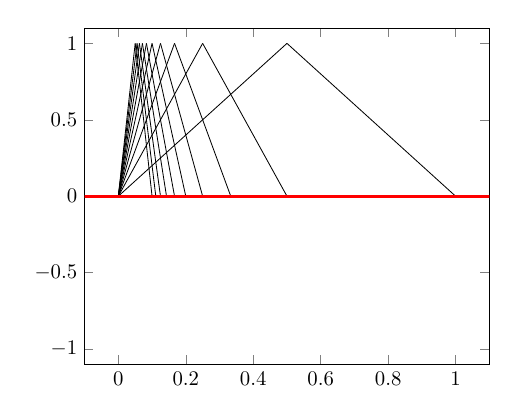
\begin{tikzpicture}[scale=.75]
          \begin{axis}[ymin=-1.1, ymax=1.1, xmin=-0.1, xmax=1.1]
            \foreach \i in {1,...,10}
            {
              \addplot[smooth,domain=0:(1/(2*\i))]{2*\i*x};
              \addplot[smooth,domain=(1/(2*\i)):(1/\i)]{2-2*\i*x};
              \addplot[smooth,domain=(1/(\i)):1.1]{0};
            }
            \addplot[smooth,color=red,ultra thick,domain=-3:3]{0};
          \end{axis}
        \end{tikzpicture}
      \end{figure}
    \end{minipage}
    \begin{minipage}{.45\textwidth}
      \[
      f_{n}: \mathbb{R} \rightarrow \mathbb{R}:\ x \mapsto
      \left\{
        \begin{array}{rl}
          2nx   & \text{ als } x \in \interval[open right]{0}{\frac{1}{2n}}\\
          2-2nx & \text{ als } x \in \interval{\frac{1}{2n}}{\frac{1}{n}}\\
          0     & \text{ als } x \in \interval[open left ]{\frac{1}{n}}{1}\\
        \end{array}
      \right.
      \]
      \[ f: \mathbb{R} \rightarrow \mathbb{R}:\ x \mapsto 0 \]
    \end{minipage}

    Merk op dat $(f_{n})_{n}$ inderdaad een rij in $A$ is.
    We beweren dat $(f_{n})_{n}$ geen convergente deelrij heeft.
    Inderdaad, kies een willekeurige deelrij $(f_{n_{k}})_{k}$ van $(f_{n})_{n}$.
    Vermits de rij $(f_{n})_{n}$ (en dus ook $(f_{n_{k}}$\stref{st:deelrij-zelfde-limiet-als-convergente-moederrij}) puntsgewijs naar de nulfunctie convergeert, is de nulfunctie de enige functie die in aanmerking komt voor de $d_{\infty}$-limiet van deze deelrij.
    Voor elke $k$ is echter $d_{\infty}(f_{n_{k}},0)$ gelijk aan $1$, dus $(f_{n_{k}})_{k}$ kan niet convergeren voor de $d_{\infty}$-metriek.
  \end{proof}
\end{tvb}

\begin{bst}
  \label{st:rijcompact-dan-volledig}
  Zij $X,d$ een metrische ruimte en $A \subseteq X$.
  Als $A$ rijcompact is, is $A$ volledig.
  
  \begin{proof}
    Zij $(x_{n})_{n}$ een Cauchyrij in $A$, omdat $A$ begrensd is, bestaat er een convergente deelrij $(x_{n_{k}})_{k}$.
    Omdat $(x_{n})_{n}$ een Cauchyrij is, zal $(x_{n})_{n}$ ook convergeren met dezelfde limiet.\stref{st:cauchy-asa-convergente-deelrij}
  \end{proof}    
\end{bst}

\begin{bst}
  \label{st:volledig-en-totaal-begrensd-dan-rijcompact}
  Zij $X,d$ een metrische ruimte en $A \subseteq X$.
  Als $A$ volledig en totaal begrensd is, is $A$ rijcompact.
  
  \begin{proof}
    Omdat $A$ totaal begrensd is, is $A$ Cauchycompact\stref{st:totaal-begrensd-dan-cauchycompact}
    Kies een willekeurige rij $(x_{n})_{n}$ in $A$.
    Omdat $A$ Cauchycompact is, bestaat er een Cauchy deelrij van $(x_{n})_{n}$.
    Omdat $A$ volledig is convergeert deze Cauchyrij.\deref{de:metrische-ruimte-volledig}
  \end{proof}
\end{bst}

\subsubsection{Compact}
\label{sec:compact}

\begin{st}
  Zij $X,d$ een metrische ruimte en $A \subseteq X$.
  $A$ is gesloten als en slechts $A$, bekeken als een metrische ruimte op zich voor de beperking van de metriek tot $A$ volledig is.
\TODO{zie oef 20, 2.7}
\end{st}

\begin{de}
  Zij $X,d$ een metrische ruimte en $A \subseteq X$.
  We noemen een verzameling $\mathcal{F}$ van open deelverzamelingen een \term{open overdekking} van $A$ als het volgende geldt:
  \[ A \subseteq \bigcup_{V \in \mathcal{F}}V \]
\end{de}

\begin{de}
  Een eindige deelverzameling van een open overdekking noemen we een \term{eindige deeloverdekking}.
\end{de}

\begin{bst}
  \label{st:rijcompact-dan-compact}
  Zij $X,d$ een metrische ruimte en $A \subseteq X$.
  Als $A$ rijcompact is, dan is $A$ compact.

  \begin{proof}
    Bewijs uit het ongerijmde:
    Stel dat er een rijcompacte deelverzameling $A$ van $X$ bestaat en een open overdekking $\mathcal{F}$ van $A$ die geen eindige deeloverdekking heeft.
    Omdat $A$ rijcompact is, is $A$ volledig\stref{st:rijcompact-dan-volledig} en totaal begrensd.\prref{pr:rijcompact-dan-totaal-begrensd}
    \begin{itemize}
    \item 
      Overdek dus $A$ met een eindig aantal open bollen met straal $\frac{1}{2}$.
      Voor minstens \'e\'en van die bollen, zeg $B_{1}$ is de doorsnede $A_{1} = B_{1} \cap A$ niet te overdekken met een eindige deelverzameling van $\mathcal{F}$.
      Als deel van een totaal begrensde verzameling is $A_{1}$ ook zelf totaal begrensd.\stref{st:deelverzameling-van-totaal-begrensd-ook-totaal-begrensd}
    \item 
      Overdek $A_{i-1}$ met een eindig aantal open bollen van straal $\frac{1}{2^{i}}$.
      Minstens \'e\'en van die bollen, zeg $B_{i}$ is de doorsnede $A_{i} = B_{i} \cap A_{i-1}$ niet te overdekken met een eindig aantal elementen van $\mathcal{F}$.
      Als deel van een totaal begrensde verzameling is $A_{i}$ ook zelf totaal begrensd.
    \item
      We verkrijgen zo een rij $(B_{n})_{n}$ van open bellen met straal van $B_{n}$ gelijk aan $\frac{1}{2^{n}}$ en een dalende rij $(A_{n})_{n}$ van open deelverzamelingen van $A$ zodat $A_{n} \subseteq B_{n}$ steeds geldt en zodat $A_{n}$ niet te overdekken is met een eindig aantal elementen van $\mathcal{F}$.
      $A_{n}$ is bovendien niet leeg.
    \end{itemize}
    Kies nu voor elke $n\in \mathbb{N}_{0}$ een $x_{n}\in A_{n}$.
    We vinden zo een rij $(x_{n})_{n}$ in $A$.
    Voor twee getallen $m,n\in\mathbb{N}$ met $m\ge n$ liggen $x_{m}$ en $x_{n}$ beide in $A_{n}$ en dus ook in $B_{n}$.
    De afstand ertussen is daarom strikt kleiner dan $\frac{1}{2^{n-1}}$.
    Dit toont aan dat $(x_{n})_{n}$ een Cauchyrij is.
    Omdat $A$ volledig is, convergeert $(x_{n})_{n}$ dus naar een bepaalde $a\in A$.
    Er geldt dan:
    \[ d(x_{n},a) \le \frac{1}{2^{n-1}} \]
    Omdat $a$ een element is van $A$ bestaat er een open deel $V$ in $\mathcal{F}$ dat $a$ bevat.
    Omdat $V$ open is, kunnen we een $n$ nemen die voldoende groot is opdat $B\left(a,\frac{1}{2^{n}}\right)$ volledig binnen $V$ ligt.
    We beweren nu dat $A_{n+2}$ ook een deel is van $B\left(a,\frac{1}{2^{n}}\right)$.
    Inderdaad, kies een $y\in A_{n+2}$ en merk op:
    \[ d(y,a) \le d(y,x_{n+2}) + d(x_{n+2},a) < \frac{1}{2^{n+1}} + \frac{1}{2^{n+1}} = \frac{1}{2^{n}} \]
    We vinden dus dat $A_{n+2}$ een deel is van $V$ en dat $A_{n+2}$ dus volledig door \'e\'en element van $\mathcal{F}$ overdekt kan worden.
    Contradictie.
  \end{proof}
\end{bst}

\begin{bst}
  \label{st:compact-dan-rijcompact}
  Zij $X,d$ een metrische ruimte en $A \subseteq X$.
  Als $A$ compact is, dan is $A$ rijcompact.

  \begin{proof}
    Kies een willekeurige rij $(x_{n})_{n}$ in $A$.
    Beschouw de rij verzamelingen $(\overline{S_{n}})_{n}$ met $S_{n} = \{x_{k}\mid k \ge n\}$.
    \begin{itemize}
    \item 
      We beweren nu dat het volgende geldt:
      \[ \left( \bigcap_{n\in \mathbb{N}_{0}}\overline{S_{n}} \right) \cap A \neq \emptyset \]
      Inderdaad, veronderstel dat de doorsnede in het linkerlid wel leeg zou zijn, dan zou $A$ een deel zijn van het complement ervan:
      \[ A \subseteq \left( \bigcap_{n\in\mathbb{N}_{0}}\overline{S_{n}}\right)^{c} = \bigcup_{n\in\mathbb{N}_{0}}\overline{S_{n}}^{c} \]
      Dit zou betekenen dat de verzameling $\{ \overline{S_{n}}^{c} \mid n \in \mathbb{N}_{0} \}$ een open overdekking van $A$ zou zijn.
      Die overdekking zou dan een eindige deeloverdekking moeten hebben.
      Er zou dus een $m\in \mathbb{N}_{0}$ moeten bestaan zodat $A$ een deel is van $\bigcup_{n=1}^{m}\overline{S_{n}}^{c}$.
      Dit zou betekenen dat de doorsnede $A \cap \bigcap_{n=1}^{m}\overline{S_{n}}$ leeg zou zijn en dat kan niet want $x_{m}$ zit er zeker in.\waarom
    \item 
      Er bestaat dus een $a\in A$ die ook in $\bigcap_{n\in\mathbb{N}_{0}}\overline{S_{n}}$ zit.
      We construeren nu een convergente deelrij van $(x_{n})_{n}$ met limiet $a$.\deref{de:rijcompact}
      Omdat $a$ in $\overline{S_{1}}$ zit, bestaat er een $n_{1} > 1$ zodat $d(a,x_{n_{1}}) < 1$ geldt.\waarom
      Omdat $a$ in $\overline{S_{n_{1}}}$ zit, bestaat er een $n_{2} > n_{1}$ zodat $d(a,x_{n_{2}}) < \frac{1}{2}$ geldt.
      Omdat $a$ in $\overline{S_{n_{k}+1}}$ zit, betsaat er een $n_{k+1} > n_{k}$ zodat $d(a,x_{n_{k}+1}) < \frac{1}{k+1}$ geldt.
      We verkrijgen zo een strikt stijgende rij $(n_{k})_{k}$ in $\mathbb{N}$ zodat $d(a,x_{n_{k}}) < \frac{1}{k}$ geldt voor elke $k\in \mathbb{N}$.
      $(x_{n_{k}})_{k}$ zal dus naar $a$ convergeren.
    \end{itemize}
  \end{proof}
\TODO{meer uitleg bij dit bewijs?}
\end{bst}



\begin{de}
  Zij $X,d$ een metrische ruimte en $A \subseteq X$, dan noemen we $A$ \term{compact} als elke open overdekking een eindige deeloverdekking heeft.
\end{de}

\begin{opm}
  Compact is dus equivalent met rijcompact.
\end{opm}

\begin{st}
  \label{st:eindig-dan-compact}
  In een metrische ruimte $X,d$ is elke eindige deelverzameling $A$ van $X$ compact.

  \begin{proof}
    Zij $V$ een willekeurige open overdekking van $A$.
    Kies dan voor elk element $a\in A$ een deelverzameling $V_{a}$ van $X$ in $V$ die $a$ overdekt.
    De unie $U$ van deze verzamelingen is dan een eindige deeloverdekking.
    \[ U = \bigcup_{a\in A}V_{a} \]
  \end{proof}
\end{st}

\begin{bpr}
  Een gesloten deel van een compact is compact.

  \begin{proof}
    Zij $K$ een compact deel van een metrische ruimte en $G$ een deel van $K$.
    Kies een willekeurige open overdekking $\mathcal{F}$ van $G$, dan is $F \cup \{G^{c}\}$ een open overdekking van $K$ (want $G$ is gesloten).
    Omdat $K$ compcat is, kunnen we een eindige deeloverdekking $\{V_{1},\dotsc,V_{n}\}$ van $\mathcal{F}$ vinden:
    \[ G \subseteq K \subseteq G^{c} \cup \bigcup_{i=1}^{n}V_{i} \]
    Duidelijk is nu dat $G$ een deel is van $\bigcup_{i=1}^{n}V_{i}$, een eindige deeloverdekking van $\mathcal{F}$ voor $G$.
  \end{proof}
\extra{bewijs via rijcompactheid}
\end{bpr}

\begin{bei}
  Zij $\mathcal{K}$ een verzameling van compacte delen van een metrische ruimte $X,d$ zodat de doorsnede van eindig veel elementen uit $\mathcal{K}$ nooit leeg is, dan is de doorsnede van alle verzamelingen uit $\mathcal{K}$ niet leeg.

  \begin{proof}
    Bewijs uit het ongerijmde: stel dat de doorsnede $\bigcap\mathcal{K}$ van de elementen van $\mathcal{K}$ leeg is.
    Noem dan $\mathcal{F} = \{K^{c}\mid K \in \mathcal{K}\}$.
    Merk op dat $\mathcal{F}$ uit open verzamelingen bestaat want elke $K$ is compact en dus gesloten.\stref{st:compact-dan-rijcompact}\stref{st:rijcompact-dan-gesloten}
    Beschouw nu een willekeurig element $K_{0} \in \mathcal{K}$.
    Omdat de unie $\bigcup_{K\in \mathcal{K}}K^{c}$ heel de metrische ruimte is, is $\mathcal{F}$ een open overdekking van $K_{0}$.
    Omdat $K_{0}$ compact is, kunnen we dus een eindig aantal verzamelingen $K_{1},\dotsc,K_{n} \in \mathcal{K}$ vinden als volgt:
    \[ K_{0} \subseteq \bigcup_{i=1}^{n}K_{i}^{c} \]
    Dit betekent echter dat de doorsnede van alle $K_{i}$ leeg is, en dat is in strijd met het gegeven.
    Contradictie.
  \end{proof}
\end{bei}
\extra{bewijs via rijcompactheid}

\begin{bpr}
  Beschouw de metrische ruimte $X,d$.
  Beschouw deelverzamelingen $A$ en $Y$ zodat $A \subseteq Y \subseteq X$ geldt.
  Noteer de beperking van $d$ tot $Y$ met $d_{Y}$.
  $A$ is compact in $X,d$ als en slechts als $A$ compact is in $Y,d_{Y}$.

  \begin{proof}
    Bewijs van een equivalentie.
    \begin{itemize}
    \item $\Rightarrow$\\
      Zij $A$ compact in $X,d$.
      Zij $\mathcal{F}$ een willekeurige overdekking van $A$ met open delen van $Y,d_{Y}$.
      Voor elke $V\in \mathcal{F}$ kunnen we een open $V'$ in $X$ kiezen zodat $V = V'\cap Y$ geldt.\prref{pr:relatief-open-snijdigen}
      Noteer $\mathcal{F}' = \{ V' \mid V \in \mathcal{F}\}$.
      $\mathcal{F}'$ is dan een overdekking van $A$ met open delen van $X$.
      Bijgevolg heeft $\mathcal{F}'$ een eindige deeloverdekking.
      Er zijn dus een eindig aantal elementen $V_{1}',\dotsc,V_{n}' \in \mathcal{F}'$ die samen $A$ overdekken.
      Wanneer we $\bigcup_{i=1}^{n}V_{i}'$ snijden met $Y$ vinden we het volgende:
      \[ A = A \cap Y \subseteq \bigcup_{i=1}^{n}V_{i} \]
      We verkrijgen een eindige deeloverdekking van $\mathcal{F}$.
      Dit toont dat $A$ compact is in $Y,d_{y}$.
    \item $\Leftarrow$\\
\TODO{bewijs:oefening}
    \end{itemize}
  \end{proof}
\end{bpr}

\begin{figure}[H]
  \centering
  \includegraphics[scale=0.5]{assets/compact.eps}
  \caption{Compactheid, een illustratie}
  \label{fig:compactheid}
\end{figure}

\subsection{Samenhangende verzamelingen}
\label{sec:samenh-verz}

\begin{de}
  We noemen een metrische ruimte $X,d$ \term{samenhangend} als enkel $\emptyset$ een $X$ open en gesloten zijn.
\end{de}

\begin{de}
  Beschouw een deelverzameling $Y$ van $X$ met $X,d$ een metrische ruimte en $d_{Y}$ de beperking van $d$ tot $Y$.
  We noemen $Y$ een \term{samenhangende deelverzameling} als en slechts als $Y,d_{Y}$ een samenhangende metrische ruimte is.
\end{de}
 
\begin{de}
  We noemen twee verzamelingen $A$ en $B$ \term{onderling gescheiden} als het volgende geldt:
  \[ A \cap \overline{B} = \emptyset = \overline{A} \cap B \]
  Merk op dat $\overline{A}$ hier de sluiting is van $A$, niet het complement.
\end{de}

\begin{bpr}
  \label{pr:karakterisatie-niet-samenhangend}
  Zij $Y$ een deelverzameling van $X$ met $X,d$ een metrische ruimte.
  $Y$ is niet samenhangend enkel als $Y$ te schrijven valt als een unie $A \cup B$ waarbij $A$ en $B$ beide niet leeg en onderling gescheiden zijn.
  In het bijzonder zijn $A$ en $B$ dan gesloten.

  \begin{proof}
    Bewijs van een equivalentie.
    \begin{itemize}
    \item $\Rightarrow$\\
      Er bestaat een gesloten deelverzameling $F$ van $X$ zodat $A = F \cap Y$ geldt.\prref{pr:relatief-gesloten-snijdigen}
      We vinden dan:
      \[ B \cap \overline{A} = B \cap \overline{F \cap Y} \subseteq B \cap F = (B \cap Y) \cap F = B \cap (Y \cap F) = B \cap A = \emptyset \]
    \item $\Leftarrow$\\
      Het is voldoende om aan te tonen dat $A$ en $B$ gesloten zijn in $Y$.
      Nu geldt:
      \[ Y \cap \overline{A} = (A \cup B) \cap \overline{A} = (A \cap \overline{A}) \cup (B \cap \overline{A}) = A \cup \emptyset = A \]
      $A$ is dus relatief gesloten in $Y$.\prref{pr:relatief-gesloten-snijdigen}
      De bewering gaat analoog op voor $B$.
    \end{itemize}
  \end{proof}
\end{bpr}

\begin{de}
  Zij $Y$ een deelverzameling van $X$ met $X,d$ een metrische ruimte.
  We noemen $Y$ \term{totaal onsamenhangend} als enkel de singletons samenhangende deelverzamelingen zijn van $Y$.
\end{de}

\begin{st}
  \label{st:singleton-samenhangend}
  Een singleton $\{x\}$, als deelverzameling van $X$ in de metrische ruimte $X,d$ is steeds samenhangend.
  
  \begin{proof}
    Enkel $\{x\}$ en $\emptyset$ zijn zowel open als gesloten.
    Er zijn bovendien geen andere mogelijke deelverzamelingen van $\{x\}$.
  \end{proof}
\end{st}

\begin{bpr}
  \label{pr:samenhangend-asa-interval}
  Een deelverzameling $Y$ van $\mathbb{R}$ is samenhangend als en slechts het een interval is.

  \begin{proof}
    Bewijs van een equivalentie.
    \begin{itemize}
    \item $\Rightarrow$\\
      Stel dat $Y$ geen interval is, dan bestaan er punten $x$,$y$ en $z$ zodat $x < z < y$ gelden met $x,y \in Y$ en $z \not\in Y$.
      Noem nu $A = \{ t \in Y \mid t < z \}$ en $B = \{ t \in Y \mid t > z \}$.
      Er geldt nu $Y = A \cup B$, $A \neq \emptyset \neq B$ en $A \cap \overline{B} = \overline{A} \cap B = \emptyset$.
    \item $\Leftarrow$\\
      Stel dat $Y$ een interval is maar niet samenhangend.
      We kunnen dan $Y$ beschrijven als $A \cup B$ met $A$ en $B$ niet leeg en $A \cap \overline{B} = \overline{A} \cap B = \emptyset$.
      Kies een $a\in A$ en $b\in B$.
      Na eventuele hernoeming geldt $a < b$.
      Noteer $C = \{ x \in A \mid x < b \}$ en stel $z=\sup C$.
      Dit supremum moet bestaan want $C$ is niet leeg ($a$ zit erin) en naar boven begrensd (door $b$).
      Duidelijk is dat $z$ tussen $a$ en $b$ ligt en omdat $Y$ een interval is moet $z$ tot $Y$ behoren.
      Bovendien behoort $z$ tot de sluiting van de verzameling $C$ waarvan het het supremum is en dus zeker $z\in \overline{A}$.
      Omdat $\overline{A} \cap B$ leeg is kan $z$ geen element zijn uit $B$ en daarom moet $z$ verschillend zijn van $b$.
      Vermits $z$ tot $Y = A \cup B$ behoort moet $z$ dus tot $A$ behoren.
      Omdat $A \cap \overline{B}$ ook leeg is kan $z$ niet in $\overline{B}$ liggen.
      Omdat $\overline{B}$ gesloten is en $z$ strikt kleiner dan $b$, kunnen we een $\delta \in \mathbb{R}_{0}^{+}$ vinden die klein genoeg is opdat $\interval[open]{z-\delta}{z+\delta}$ een deel is van $C$.
      Het supremum van $C$ zou dus strikt groter moeten zijn dan $z$, wat strijdig is met de definitie van $z$.
      Contradictie.
    \end{itemize}
  \end{proof}
\end{bpr}

\begin{bpr}
  \label{pr:convexe-deelverzamelingen-samenhangend}
  Zij $\mathbb{R},V,+, \|\cdot\|$ een genormeerde vectorruimte.
  Alle convexe deelverzamelingen van $V$ zijn samenhangend voor de metriek ge\"induceerd door $\|\cdot\|$.

  \begin{proof}
    Stel dat $Y$ een niet-leeg convex deel is van $V$ maar niet samenhangend.
    $Y$ valt dan te schrijven als $A \cup B$ met $A$ en $B$ elk niet leeg en $A \cap \overline{B} = \overline{A} \cap B = \emptyset$.
    Kies een $x\in A$ en een $y\in B$ en benoem $S$ en $T$ als volgt:
    \[ S = \{ t\in \interval{0}{1} \mid (1-t)x + ty \in A \} \]
    \[ T = \{ t\in \interval{0}{1} \mid (1-t)x + ty \in B \} \]
    $S$ en $T$ zijn dan niet leeg want $0 \in S$ en $1 \in T$ gelden.
    Omdat $Y$ convex is zal $\interval{0}{1}$ de unie zijn van $S$ en $T$.
    Als $t\in S \cap \overline{T}$ zit, dan bestaat er een rij $(t_{n})_{n}$ in $T$ met $t$ als limiet.
    Dan zal echter de rij $\left((1-t_{n})x + t_{n}y\right)$ convergeren naar $(1-t)x + ty$ in $V$ en zal dus $(1-t)x+ty$ een element zijn van $\overline{B}$.
    Omdat $t$ ook in $S$ zit zou $(1-t)x+ty$ een element zijn van $A \cap \overline{B}$.
    Analoog bewijst met dat $\overline{S} \cap T$ leeg is.
    Dit zou dat betekenen dat $\interval{0}{1}$ niet samenhangend is.
    Contradictie.\prref{pr:samenhangend-asa-interval}
  \end{proof}
\end{bpr}

\begin{bpr}
  \label{pr:niet-disjunctie-samenhangende-unie-samenhangend}
  In een metrische ruimte $X,d$ is de unie van niet-disjunctie samenhangende verzamelingen samenhangend.

  \begin{proof}
    Zij $\bigcup S$ de unie van een verzameling onderling niet disjuncte verzamelingen.
    Bewijs uit het ongerijmde: Stel dat $\bigcup S$ niet samenhangend is.\\
    $\bigcup S$ valt dan te schrijven als $A \cup B$ met $A$ en $B$ niet elk leeg en $A \cap \overline{B} = \overline{A} \cap B = \emptyset$.
    Voor elke $Y = (A \cap Y) \cup (B \cap Y)$ in $S$ merken we op: 
    \[ (A \cap Y) \cap \overline{(B \cap Y)} \subseteq A \cap \overline{B} = \emptyset \]
    Analoog vinden we dit:
    \[ \overline{(A \cap Y)} \cap (B \cap Y) \subseteq \overline{A} \cap B = \emptyset \]
    Omdat $Y$ samenhangend is, zal ofwel $A \cap Y$ leeg zijn ofwel $B \cap Y$.
    Kies nu een $x\in \bigcap S$, dan behoort $x$ ofwel tot $A$, ofwel tot $B$, want $A$ en $B$ zijn disjunct.
    Na eventuele hernoeming kunnen we stellen dat $x$ tot $A$ behoort.
    $x$ is dan een element van $A \cap Y$ voor elke $Y$ en dus is $B \cap Y$ leeg voor elke $Y$.
    Dit impliceert dat $B$ leeg is.
    Contradictie.
  \end{proof}
\end{bpr}

\begin{bpr}
  Beschouw een willekeurige deelverzameling $Y$ van een metrische ruimte $X,d$.
  Voor elke $x\in Y$ bestaat er een grootste samenhangende deelverzameling $Y_{x}$ die $x$ bevat en deel is van $Y$.
  Voor elk paar $x$ en $y$ in $Y$ zal dan $Y_{x} \cap Y_{y}$ leeg zijn of $Y_{x} = Y_{y}$ gelden.
  $Y$ is de unie van twee aan twee disjunctie samenhangende deelverzamelingen.

  \begin{proof}
    Kies $x\in Y$ en noteer met $S$ de verzameling van alle samenhangende deelverzamelingen van $Y$ waar $x$ toe behoort.
    Noteer $Y_{x} = \bigcup S$.
    Per definitie is $\bigcap S$ niet leeg.
    $Y_{x}$ is nog steeds samenhangend.\prref{pr:niet-disjunctie-samenhangende-unie-samenhangend}
    Het is duidelijk de grootste samenhangede deelverzameling van $Y$ waar $x$ in zit.
    Neem nu $x,y\in Y$ en stel dat $Y_{x}\cap Y_{y}$ leeg is, dan is $Y_{x}\cup Y_{y}$ een samenhangende deelverzameling van $Y$ waar $x$ en $y$ in zitten.
    Er geldt dus $Y_{x} \cup Y_{y} \subseteq Y_{x}$ en $Y_{y} \cup Y_{x} \subseteq Y_{y}$.
    Dit impliceert dat $Y_{x}$ en $Y_{y}$ gelijk zijn.
  \end{proof}
\end{bpr}

\begin{bpr}
 Als $Y$ een open deel is van $\mathbb{R}^{p}$, dan zijn de samenhangende componenten van $Y$ weer open.

 \begin{proof}
   Kies een $x\in Y$ en beschouw de samenhangende component $Y_{x}$ van $x$ in $Y$.
   Kies een $a\in Y_{x}$.
   Omdat $a$ tot $Y$ behoort, bestaat dan een $\delta \in \mathbb{R}_{0}^{+}$ met $B(a,\delta) \subseteq Y$.
   Omdat $B(a,\delta)$ samenhangend is en het punt $a$ gemeen heeft met $Y_{x}$ moet $B(a,\delta)$ een deel zijn van $Y_{x}$.
 \end{proof}
\end{bpr}

\end{document}

%%% Local Variables:
%%% mode: latex
%%% TeX-master: t
%%% End:
